%%%%%%%%%%%%%%%%%%%%%%%%%%%%%%%%%%%%%%%%%%%%%%%%%%%%%%%%%%%%%%%%%
% Lecture date: 19-11-25
%%%%%%%%%%%%%%%%%%%%%%%%%%%%%%%%%%%%%%%%%%%%%%%%%%%%%%%%%%%%%%%%%
\chapter{Scattering Theory}
\section{Non-relativistic Perturbation Theory}
Quantum states are eigenfunctions of (bare) Hamiltonians. They should be (complete) orthonormal basis for the Hilbert space.
\begin{align*}
   H_0 \phi_n = E_n \phi_n \\
   \int \dd[3]{x} \phi^*_m \phi_n = \delta_{mn} \\
\end{align*}

Schrödinger equation 
\begin{align*}
   (H_0 + V) \psi = i \dv{\psi}{t} \label{math:sch}
\end{align*}

Make the ansatz that an arbitrary state is a superposition of of $\phi_n$
\begin{align}
   \psi = \sum a_n(t) \phi_n (\pmb{x}) \euler^{-iE_n t}
\end{align}
Insert it into Schrödinger equation \ref{math:sch}
\begin{align*}
   i\sum \dv{a_n}{t} \phi_n (\pmb x) \euler^{-iE_n t} &= \sum V(\pmb x, t) a_n (t) \phi_n(\pmb{x}) \euler^{-iE_n t}
   \shortintertext{multiply by $\phi^*_f(\pmb x)$ and $\int \dd[3]{x}$}
   \dv{a_f}{t} &= -i \sum_n a_n(t) \int \dd[3]{x} \phi^*_f V \phi_n \cdot \euler^{i(E_f - E_n)t }
\end{align*}

Assume this potential acts for a finite time $T$, between $[-T/2, T/2]$.

The initial state is $\ket{i}$ and eigenstate of $H_0$. 
\begin{align*}
   a_i (-T/2) &= 1 \\ 
   a_n(-T/2) &= 0 \;  \text{ with }n \neq i \\
\end{align*}
\begin{align}
   \dv{a_f}{t} &= -i  a_n(t) \int \dd[3]{x} \phi^*_f V \phi_i \cdot \euler^{i(E_f - E_i)t } \label{math:nonRelPertAf}\\
   \shortintertext{integrate}
   a_f (t) &= -i \eval{\int_{-T/2}^t \dd{t'} \int \dd[3]{x} \phi^*_f V \phi_i \euler^{i(E_f - E_i)t}}_{t=-T/2} \notag
\end{align}

\begin{align}
   T_{fi} &= a_f(T/2) \notag \\
   &= -i \int_{-T/2}^{T/2} \dd{t} \int \dd[3]{x} \left[ \phi_f(\pmb{x}) \euler^{-iE_f t} \right]^* V(\pmb x, t) \left[ \phi_i(\pmb x) \euler^{-iE_i t} \right] \notag \\
   T_{fi} &= -i \int \dd[4]{x} \phi^*_f (x) V(x) \phi_i (x)
\end{align}
for $a_f(t) \ll 1$.

Assume static potential $V(x) = V(\pmb x)$
\begin{align}
   \begin{split}
    T_{fi} &= -i V_{fi} \int^{+\infty}_{-\infty} \dd{t} \euler^{-i(E_f - E_i)t}\\
          &= -2\pi i V_{fi} \delta(E_f - E_i) \\
   V_{fi} &= \int \dd[3]{x} \phi_f^*(\pmb x) V(\pmb{x}) \phi_i(\pmb x)
   \end{split}
\end{align}

As $\Delta E \rightarrow 0$, $\Delta t = \infty$, so infinite time is needed to get from $\ket{i} \rightarrow \ket{f}$. Define transition probability per unit time
\begin{align}
   W &= \lim_{T \rightarrow \infty} \frac{|T_{fi}|^2}{T} \notag \\
     &= \lim_{T \rightarrow \infty} 2 \pi \frac{|V_{fi}|^2}{T} \delta(E_f - E_i) \int_{-T/2}^{T/2} \dd{t} \euler^{i(E_f - E_i)t} \notag\\
     &= \lim_{T \rightarrow \infty} 2 \pi \frac{|V_{fi}|^2}{T} \delta(E_f - E_i) T \notag\\
     &= 2\pi |V_{fi}|^2 \delta(E_f - E_i) \label{math:deltaSqaure}
\end{align}

It is only meaningful after integration over initial and final states. In collider initial state is prepared with fixed momentum $\pmb{p_e}$. So no integration over initial states.  For proton (hadron), it is a bit more complicated since the quarks are moving inside of proton.

Define the density of final states $\rho(E_f)$. \underline{Fermi's Golden rule}
\begin{align}
   \begin{split}
      W_{fi} &= 2 \pi \int \dd{E_f} \rho(E_f) |V_{fi}|^2 \delta(E_f - E_i) \\
   &= 2 \pi |V_{fi}|^2 \rho(E_i)
   \end{split}
\end{align}

The result can be improved by considering higher order scatterings, i.e.~scatter multiple times. For each order insert the result for $a_f(t)$  into formula (\ref{math:nonRelPertAf}) for the $a_{n \neq i} (t)$
\begin{align}
   \dv{a_f}{t} = - \sum a_n (t) \int \dd \phi^*_f V\phi_n \dd[3]{x} \euler^{i(E_f - E_i)t}
   \shortintertext{replace}
   a_n(t) = -i \int_{T/2}^{t}\dd{t'} \int \dd[3]{x'} \phi^*_n V \phi_i \euler^{i(E_n - E_i)t} 
\end{align}

Then
\begin{align*}
   \dv{a_f}{t} = -i \int \dd[3]{x} \phi^*_f V \phi_i \euler^{i(E_f - E_i)t} + (-i)^2 \sum_{n \neq i} \int_{-T/2}^{t} \dd{t'} \euler^{i (E_n - E_i)t'} V_{fn} \euler^{i(E_f - E_n)t}
\end{align*}

Correlation to $T_{fi}$
\begin{align*}
   T_{fi} &= \dots - \sum_{n \neq i} V_{fn} V_{ni} \int_{-\infty}^{+\infty} \dd{t} \euler^{i(E_f - E_n)t} \int_{-\infty}^{t} \dd{t'} \euler^{i(E_n - E_i)t}
   \shortintertext{regulate the last exponential by adding a small constant $\epsilon$}
   T_{fi} &= \dots - 2\pi i \sum_{n \neq i} \frac{V_{fn} V_{ni}}{E_i - E_n + i \epsilon} \delta(E_f - E_i)
\end{align*}
This is second order in perturbation theory including time dependence.

We can treat it like Feynman diagram with vertex  $V_{ni}$ and propagator $1/(E_i - E_n + i\epsilon)$. 

It is not manifestly covariant. Potential is assumed static and it defines the preferred reference frame. To go to relativistic formulation, consider other particle(s), which create electromagnetic potential for first particle to scatter in and vice versa.

\section{Scalar Electrodynamics}
\subsection{Complex scalar}
\begin{align}
   \lag = (\partial_mu \phi)^* (\partial^\mu \phi) - m^2 \phi^* \phi
\end{align}

It has the equation of motion
\begin{align}
   (\partial^2 + m^2) \phi = 0
\end{align}

To include electromagnetism consider generalized momentum 
\begin{align*}
   p^\mu &\mapsto p^\mu +_ e A^\mu  \\
   i \partial^\mu &\mapsto i \partial^\mu + e A^\mu
\end{align*}
Insert it into equation of motion
\begin{align}
   \begin{split}
    (\partial^2 + m^2) \phi &= - V\phi \\
   V &= -ie (\partial_\mu A^\mu + A^\mu \partial_mu) - e^2 A^2
   \end{split}
\end{align}

Fine structure constant $\alpha = e^2/(4\pi) \approx 1/137 \ll 1$. So in first order drop the $e^2$ term.
\begin{align}
   T_{fi} &= -i \int \dd[4]{x} \phi^*_f{x} V(x) \phi_i(x) \notag \\
          &= -i \int \dd[4]{x} \phi^*_f(x) ie \left[ \partial_\mu A^\mu + A^\mu \partial_\mu  \right] \phi_i (x) \notag
   \shortintertext{integrate by parts and drop surface terms}
          &= -i \int j_\mu^{fi} A^\mu \dd[4]{x} \label{math:TJA}
\end{align}
with the current
\begin{align}
   j_\mu^{fi} (x) = -ie \left[ \phi^*_f (\partial_\mu \phi_i) - (\partial_\mu \phi_f)^* \phi_i \right]
\end{align}
The current is conserved for free field $\partial_\mu j^\mu (x) = 0$

Write $\phi_i$ and $\phi_f$ as plane waves
\begin{align*}
   \phi_i (x) &= N_i \euler^{-ip_i \cdot x} \\
   j_\mu^{fi} &= -e N_i N_f (p_i + p_f) \euler^{i (p_f - p_i) \cdot x}
\end{align*}

\subsection{Scalar Charged Scattering}
Consider potential for particle 1 to scatter caused by particle 2 and vice versa.
\begin{align*}
   \feynmandiagram[vertical=v1 to v2]{
      pa[particle=\(p_A\)] -- [fermion] v1 -- [fermion] pc[particle=\(p_C\)],
      pb[particle=\(p_B\)] -- [fermion] v2 -- [fermion] pd[particle=\(p_D\)],
      v1 -- [photon, edge label=\(\gamma\)] v2,
   };
\end{align*}

What potential $A_\mu$ does $j_\mu^{(2)}$ create for particle 1 to scatter in inhomogeneous Maxwell equation
\begin{align*}
   \partial^2 A^\mu = j^{\mu(2)} = -e N_B N_D (p_D + p_B)^\mu \euler^{i(p_D - p_B)\cdot x}
\end{align*}

Also consider photons as plane waves
\begin{align}
   \partial^2 \euler^{iqx} = -q^2 \euler^{iqx} \notag
   \shortintertext{thus}
   A^\mu = - \frac{1}{q^2} j^{\mu (2)}
\end{align}
with $q = p_D - p_B$.

Insert into \ref{math:TJA} 
\begin{align*}
   T_{fi} &= -i \int j_\mu^{(1)} (x) \left(-\frac{1}{q^2} \right) j^{\mu (2)} (x) \dd[4]{x} \\
          &= -i e^2 N_A N_B N_C N_D \int \dd[4]{x} \euler^{i(p_c + p_D - p_A - p_B)} (p_C + p_A)_\mu (p_D + p_B)^\mu \frac{-1}{q^2} \\
          &= -i N_A N_B N_C N_D (2\pi)^4 \delta^{(4)} (p_C + p_D - p_A - p_B) \M
   \shortintertext{The invariant matrix element}
   -i\M &= ie (p_A + p_C)^\mu \left( -i \frac{g_{\mu\nu}}{q^2}  \right) ie (p_B + p_D)^\nu
\end{align*}
It is symmetric in $(A,C)$ and $(B,D)$.

\subsection{From Amplitude to Cross Section}
In the laboratory we measure cross sections. Need to fix norm, $\phi = N \euler^{-ipx}$. The number density is defined by
\begin{align}
   \rho = 2 E |N|^2
\end{align}
The infinitesimal number of particles $\rho \dd[3]{x}$ is Lorentz invariant. Norm is chosen as
\begin{align}
   \int \rho \dd{V} = 2E
\end{align}

We are interested in Transition rate per unit time and volume. 
\begin{align*}
   W_{fi} &= \frac{|T_{fi}|^2}{T \cdot V} \\
   T_{fi} &= -i N_A N_B N_C N_D (2\pi)^4 \delta^{(4)}(p_c + p_D - p_A - p_B) \M
\end{align*}

Same trick as before (\ref{math:deltaSqaure}) to get rid of one of $\delta$
\begin{align*}
   \int \dd[4]{x} &= T \cdot V  \\
   W_{fi} &= \frac{1}{V^4} (2\pi)^4 \delta^{(4)} (p_C + p_D - p_A - p_B) |\M|^2
\end{align*}

Definition of cross section
\begin{align}
   \sigma = \frac{W_{fi}}{\text{initial flux}} \cdot (\text{number of final states})
\end{align}
Imagine particles in a box
\begin{align*}
   (\text{number of final state particles}) = \frac{V \dd[3]{p}}{(2\pi)^3 2 E}
\end{align*}

Density of incoming particles A  $2E_A / V$. The box has length $\pmb{v}_A \cdot t$. Number of beam particles passing through unit area $A$ per unit time is $\pmb{v}_A \cdot t 2 E_A/(V t)$.  Particle B (target). Initial flux is $|\pmb{v}_A| \frac{2E_a}{v} \frac{2E_B}{V}$
\begin{align*}
   \dd{\sigma} &= \frac{V^2}{|\pmb{v}_A| 2 E_A 2 E_B} \frac{1}{V^4} |M|^2 \frac{(2\pi)^4}{(2\pi)^4} \delta^{(4)} (p_c + p_D - p_A - p_B) \frac{\dd[3]{p_C}}{2\pi} \frac{\dd[3]{p_D}}{2\pi} V^2 \\
               &= \frac{|\M|^2}{F} \dd{Q}
\end{align*}
with $F = |\pmb{v}_A| 2 E_A 2 E_B$ and $\dd{Q} = (2\pi)^4 \delta^{(4)}(p_C + p_D - p_A - p_B) \frac{\dd[3]{p_C}}{(2\pi)^3 2E_C} \frac{\dd[3]{p_D}}{(2\pi)^3 2 E_D}$and $B$ at rest.

If both are moving $F = |\pmb{v}_A - \pmb{v}_B| 2 E_A 2E_B = 4 \sqrt{(p_A \cdot p_B)^2 - m_A^2 m_B^2 }$.

In centre of mass system
\begin{align}
   \dv{\sigma}{\Omega} = \frac{1}{64 \pi^2 s } \frac{p_f}{p_i} |M|^2 
\end{align}

For $e \mu$ scattering 
\begin{align*}
   \dv{\sigma}{\Omega} = \frac{\alpha^2}{4s} \left( \frac{3 + \cos(\theta)}{1 - \cos(\theta)} \right)
\end{align*}
with $\theta$ angle between $\pmb{p}_A$ and $\pmb{p}_C$.

Also it includes decays, for example $n \rightarrow p e^- \bar{\nu}_e$.

%%%%%%%%%%%%%%%%%%%%%%%%%%%%%%%%%%%%%%%%%%%%%%%%%%%%%%%%%%%%%%%%%
% Lecture date: 19-11-26
%%%%%%%%%%%%%%%%%%%%%%%%%%%%%%%%%%%%%%%%%%%%%%%%%%%%%%%%%%%%%%%%%
\paragraph{Decay versus cross section}
Examples are $\pi^- \rightarrow \mu^- \bar{\nu}_\mu$, $t \rightarrow W^+ b$

\begin{align}
   \dd{\Gamma} &= \frac{1}{2E_A} |\M|^2 \frac{\dd[3]p_1}{(2\pi)^3 2 E_1}\frac{\dd[3]p_2}{(2\pi)^3 2 E_2} \\
   \Gamma &= \int \dd{\Gamma}
\end{align}

Pion for instance has different decay modes.
\begin{align}
   \Gamma_\text{tot} = \Gamma(\pi \rightarrow \mu \nu_\mu) + \Gamma(\pi \rightarrow e \bar{\nu}_e)
\end{align}

Radioactive decay 
\begin{align}
   N_A (t) = N(0) \euler^{-\Gamma_{\text{tot}}t}
\end{align}

Lifetime is defined as 
\begin{align}
   \tau_A = 1/\Gamma_\text{tot}(A)
\end{align}

\section{Electron Electron scattering}
\begin{align*}
   \feynmandiagram[vertical=v1 to v2]{
      i1[particle=\(e^-\)] --[momentum'=\(p_A\)] v1 --[momentum'=\(p_C\)] f1[particle=\(e^-\)],
      i2[particle=\(e^-\)] --[momentum=\(p_B\)] v2 --[momentum=\(p_D\)] f2[particle=\(e^-\)],
      v1 --[photon, edge label=\(\gamma\)] v2,
   };
   \quad
   \begin{tikzpicture}
      \begin{feynman}
      \diagram [vertical=a to b] {
         i1 [particle=\(e^{-}\)] --[momentum'=\(p_A\)]  a -- [draw=none] f1 [particle=\(e^{-}\), label=0:\(p_C\)],
         i2 [particle=\(e^{-}\)] --[momentum=\(p_B\)]  b -- [draw=none] f2 [particle=\(e^{-}\), label=0:\(p_D\)],
         a -- [photon, edge label'=\(\gamma\)] b,
      };
      \diagram* {
         (a) --  (f2),
         (b) --  (f1),
      };
      \end{feynman}
   \end{tikzpicture}
\end{align*}

One cannot differentiate electron from electron. We have to add both diagrams before squaring
\begin{align*}
-iM_{e^- e^-} = -i e^2 \left[ - \frac{(p_A + p_C)_\mu \cdot (p_B + p_D)^\mu}{(p_D - p_B)^2} - \frac{(p_A + p_D)_\mu \cdot (p_B + p_C)^\mu}{(p_C - p_B)^2}\right]
\end{align*}

\section{Electron Positron scattering}
\begin{align*}
      \feynmandiagram[vertical=v1 to v2]{
      i1[particle=\(e^-\)] --[momentum'=\(p_A\)] v1 --[momentum'=\(p_C\)] f1[particle=\(e^-\)],
      i2[particle=\(e^+\)] --[momentum=\(p_B\)] v2 --[momentum=\(p_D\)] f2[particle=\(e^+\)],
      v1 --[photon, edge label=\(\gamma\)] v2,
   };
   \quad
   \feynmandiagram[horizontal=v1 to v2]{
      i1[particle=\(e^-\)] --[momentum'=\(p_B\)] v1 --[reversed momentum'=\(p_A\)] f1[particle=\(e^-\)],
      i2[particle=\(e^-\)] --[reversed momentum=\(p_D\)] v2 --[momentum=\(p_C\)] f2[particle=\(e^-\)],
      v1 --[photon, edge label=\(\gamma\)] v2,
   };
\end{align*}

\section{Mandelstam Variables}
Only for two-to-two scattering
\begin{align}
   s &= (p_A + p_B)^2 \\
   u &= (p_A - p_C)^2 \\
   t &= (p_A - p-D)^2 
\end{align}

Diagrams are often classified by the momentum of propagator. Mandelstam variables $s$, $t$ and $u$ are not independent.
\begin{align}
   s + u + t = \sum m_i^2
\end{align}

One can set the reference frame such that
\begin{align*}
   p_A &= (E,0,0,E) \\
   p_B &= (E,0,0,-E) \\
   p_C &= (E,0,E \sin(\theta), E\cos(\theta)) \\
   p_D &= (E, 0, -E \sin(\theta), -E\cos(\theta))  
\end{align*}
Then 
\begin{align}
   s &= 4 E^2 \\
   t &= -\frac{s}{2}(1-\cos(\theta)) \\
   u &= -\frac{s}{2} (1+\cos(\theta))
\end{align}

\section{Origin of the propagator}
Non-relativistically 
\begin{align}
   T_{fi}^{(2)} = -i \sum_{n \neq i} V_{fn} \frac{1}{E_i - E_n} V_{ni} 2\pi \delta(E_f - E_i)
\end{align}

Electron positron scattering
each Feynman diagram is the sum of all possible time orderings in old fashioned perturbation theory. 

Two times orderings for s-channel diagram
\begin{align*}
   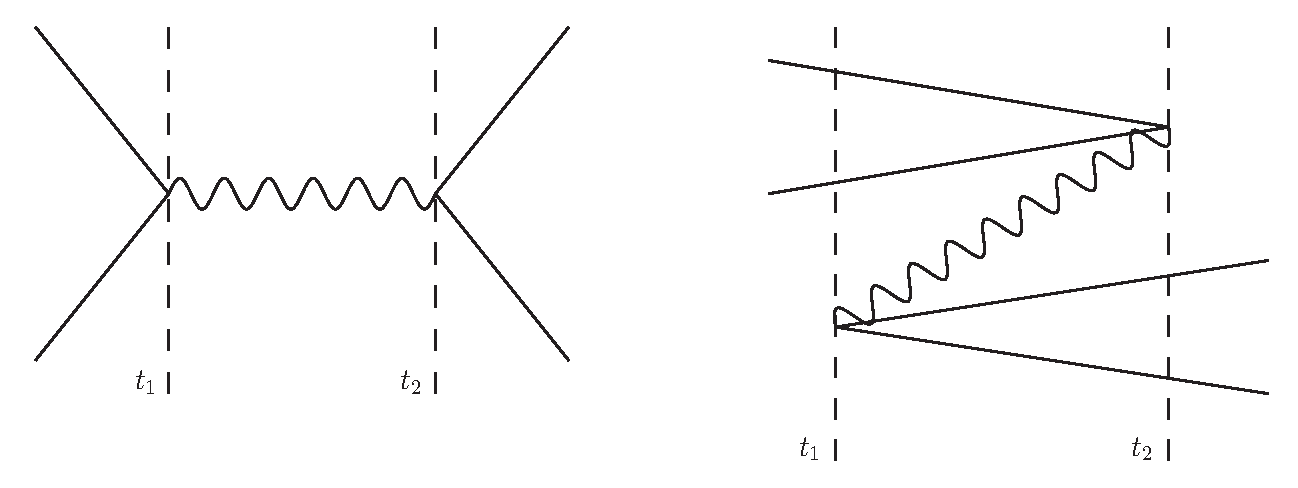
\includegraphics[width=0.8\linewidth]{propTime/1.eps}
\end{align*}
(one can understand the second diagram by saying that an amount of energy is borrowed to produce particle pair.)

\begin{align*}
   \M &\sim V_{fn} \frac{1}{E_i - E\gamma} V_{ni} + V_{fn} \frac{1}{E_i - 2E_i - E_\gamma} V_{ni} \\
      &= V_{fn} \frac{2E_\gamma}{E_i^2 - E_\gamma^2} V_{ni}
\end{align*}

\begin{align*}
   (p_A + p_B) ^2 &= E_i^2 - (\pmb{p}_A + \pmb{p}_B)^2  \\
   E_\gamma^2 &= \pmb{p}^2 + m_\gamma^2 \\
   p &= p_A + p_B \\
   \frac{1}{E_i^2 - E_\gamma^2} &= \frac{1}{(p_A + p_B)^2 - m_\gamma^2} = \frac{1}{q^2}
\end{align*}

\section{Electron interacting with $A^\mu$}
\begin{align}
   (ip_\mu \gamma^\mu - m) \psi =0\\
   \psi = u(\pmb{p}) \euler^{-i p \cdot x}
\end{align}

Consider $p^\mu \mapsto p^\mu + eA^\mu$
\begin{align*}
   (\gamma^\mu p_\mu - m) \psi = (\gamma^0 V) \psi \\
   \gamma^0 V = -e \gamma_\mu A^\mu
\end{align*}

\begin{align*}
   T_{fi} &= -i \int \dd[4]{x} \psi_{f}^\dagger (x) V(x) \psi_i (x) \\
          &= ie \int \dd[4]{x} \overline{\psi}_f (x) \gamma_\mu A^\mu \psi_i  \\
          &= -i \int \dd[4]{x} j_\mu^{fi} A^\mu 
\end{align*}

\begin{align}
   j_\mu^{fi} &= -e \bar\psi _f \gamma_\mu \psi_i = -e \bar{u}_f \gamma_\mu u_i \euler^{i(p_f - p_i)x}
   \shortintertext{In non-relativistic case}
   j_\mu^{fi} &= -e \bar\psi _f \gamma_\mu \psi_i = -e (p_f + p_i)_\mu \euler^{i(p_f - p_i)x}
\end{align}
So we have Feynman rules for external fermions and vertex.

One can write the following identity
\begin{align}
   \bar{u}_f \gamma^\mu u_i = \frac{1}{2m} \bar{u}_f \left[ (p_f + p_i)^\mu + i \sigma^{\mu\nu} (p_f - p_i)_\nu \right] u_i
\end{align}
with $\sigma^{\mu\nu} = \frac{i}{2} [\gamma^\mu, \gamma^\nu]$. First term is exactly we have before. It comes from electric charge interaction. The second part is then spin or magnetic interaction. It can be shown that $j^\mu A_\mu$ in Non-relativistic limit becomes $\pmb{\sigma} \cdot \pmb{B}$ from $\sigma^{\mu\nu}$ term.

\section{Møller Scattering}

%TODO: Diagrams s, t, u
$e^- e^- \rightarrow e^- e^-$

\begin{align*}
   T_{fi} &= -i \int \dd[4]{x} j_\mu^{(1)} (-\frac{1}{q^2}) j_2^\mu (x) \\
          &= -i (-e \bar{u}_c \gamma_\mu u_A) \left( -\frac{1}{q^2} \right) (-e\bar{u}_D \gamma^\mu u_B) (2\pi)^4 \delta^{(4)}(p_A + p_B - p_C - p_D)
   \shortintertext{with $q = p_A - p_C = p_D - p_B$}
          &= -i (2\pi)^4 \delta^{(4)} (p_A + p_B - p_C - p_D) \M
\end{align*}

\begin{align*}
   -i\M = (ie \bar{u}_C \gamma^\mu u_A) \left( \frac{-ig_{\mu\nu}}{q^2}  \right) \left( ie \bar{u}_D \gamma^\nu u_B \right)
\end{align*}
swapping order of final state electrons. Minus sign comes from electron being fermion.

\begin{align*}
   \M = \M_1 + \M_2 = -e^2 \frac{(\bar{u}_C \gamma^u u_A)(\bar{u}_D \gamma_\mu u_B) }{(p_A - p_C)^2} + e^2 \frac{(\bar{u}_D \gamma^u u_A)(\bar{u}_C \gamma_\mu u_B) }{(p_A - p_D)^2}
\end{align*}

\begin{align}
   |\M|^2 &= |\M_1|^2 + |\M_2|^2 + 2 \Re(\M_1 \M_2^*) \\
   |\M_1|^2 &=  \frac{e^4}{t^2} (\bar{u}_C \gamma^\mu u_A) (\bar{u}_A \gamma^\nu u_D) (\bar{u}_D \gamma_\mu u_B) (\bar{u}_B \gamma_\nu u_D)
\end{align}

Most experiments are done without polarized beams. Thus we must average incoming spins.
\begin{align}
   \frac{1}{(2S_A + 1) (2S_B + 1) } \sum_{S_A, S_B}
\end{align}
We should also sum over the final states (if it will not be observed).

Shuffle the spinors and use spin sum identities
\begin{align}
   \sum_{S} u^{(S)}(p) \bar{u}^{(S)}(p) = \slashed{p} + m
\end{align}
we get (for the second half)
\begin{align*}
   \tr[(\slashed{p}_D + m) \gamma^\mu (\slashed{p}_B + m)\gamma^\nu]
\end{align*}

\begin{align*}
   \frac{1}{4} \sum_{\text{spin}} |\M_1|^2 = \frac{e^4}{4t^2} \tr[(\slashed{p}_D + m) \gamma^\mu (\slashed{p}_B + m)\gamma^\nu]   \tr[(\slashed{p}_C + m) \gamma^\mu (\slashed{p}_A + m)\gamma^\nu]
\end{align*}

We know the trace of odd number of gamma matrices vanished. Thus
\begin{align*}
   &\frac{4e^4}{t^2} \big[ 2 p_A \cdot p_D p_C \cdot p_B + 2 p_A \cdot p_Be p_C \cdot p_D -4 p_A \cdot p_C p_B \cdot p_D + 4 p_A \cdot p_C p_B \cdot p_D + \\
   &\quad m^2 (2p_B \cdot p_D -4 p_B\cdot p_D + 2p_A \cdot p_C - 4 p_A \cdot p_C) + 4m^4 \big]
   \shortintertext{In most experiments, center of mass energy is well above electron mass, thus we can set $m_e = 0$}
   &= 8 (u^2 + s^2)
\end{align*}

\begin{align*}
   s &= 2 p_A \cdot p_B = 2 p_C \cdot p_D \\
   t &= -2 p_A \cdot p_C \\
   u &= -2 p_A \cdot p_D
\end{align*}

Correspondingly
\begin{align*}
   \frac{1}{4} \sum |\M_2|^2 = \frac{2e^4}{u^2} (t^2 + s^2)
\end{align*}

In interference term, there is just one (long) trace.
\begin{align*}
   \frac{1}{4} \sum 2 \Re(\M_1 \M_2^*) = \frac{4e^4}{t u }s^2
\end{align*}

\begin{align*}
   \frac{1}{4} \sum |\M|^2 &= \overline{|\M|^2} \\
                           &= 2e^4 \left[ \frac{u^2 + s^2}{t^2} + \frac{t^2 + s^2}{u^2} + 2 \frac{s^2}{tu} \right]
\end{align*}

%%%%%%%%%%%%%%%%%%%%%%%%%%%%%%%%%%%%%%%%%%%%%%%%%%%%%%%%%%%%%%%%%
% Lecture date: 19-12-03
%%%%%%%%%%%%%%%%%%%%%%%%%%%%%%%%%%%%%%%%%%%%%%%%%%%%%%%%%%%%%%%%%
$e^- \mu^- \rightarrow e^- \mu^-$

$e^- e^+ \rightarrow \mu^+ \mu^-$
Change $k' \rightarrow -p$ and $s \leftrightarrow t$.
\begin{align*}
   \dv{\sigma}{\Omega} &= \frac{\alpha^2}{4s} (1+\cos^2 \theta)
   \shortintertext{integrate over solid angle}
                       &= \frac{4\pi \alpha^2}{3s}
\end{align*}
Cross section drops down with $1/s$. With high luminosity we can evade the problem.

\section{Photons and Polarization Vectors}
Photon field $A^\mu (x)$ satisfies Maxwell equations
\begin{align*}
   \partial^2 A^\mu = j^\mu
\end{align*}
Even in classical theory, there is gauge freedom. With Lorenz condition $\partial_\mu A^\mu = 0$ there is still some gauge freedom.

\begin{align}
   A_\mu \mapsto A'_\mu = A_\mu + \partial_\mu \Lambda(x)  \label{math:gaugeLambda}
\end{align}
if $\partial^2 \Lambda (x) = 0$. 

Free photon 
\begin{align}
   \partial^2 A^\mu &= 0 \\
   A^\mu &= \epsilon^\mu (\pmb{q}) \euler^{-iq\cdot x}
\end{align}
with $\epsilon(\pmb p)$ polarization vector with $\mu =0, 1,2,3$. Thus equation for polarization vector is
\begin{align}
   q^2 \epsilon^\mu (\pmb{q}) \euler^{-i q \cdot x} = 0
\end{align}
with $q^2 = m_\gamma^2 = 0$.

From QM, we know for spin $1$ particle, $S_z = +1, 0, -1$. With Lorenz condition, 
\begin{align*}
   q_\mu \epsilon^\mu = 0
\end{align*}
thus there are three independent components.

We still have constraint \ref{math:gaugeLambda}. To make it specific, choose
\begin{align}
   \Lambda = i a \euler^{-iq \cdot x}
\end{align}
then the constraint is satisfied
\begin{align*}
   \partial^2 \Lambda = q^2 \Lambda = 0
\end{align*}
Use this specific $\Lambda$, the transformation of $A_\mu$ becomes
\begin{align}
   A_\mu \mapsto A'_\mu = A_\mu + \partial_\mu \Lambda \\
   \epsilon \euler^{-iq\cdot x} \mapsto \epsilon' \euler^{-iq\cdot x} = \epsilon \euler^{-iq\cdot x} + ia (-i) q_\mu \euler^{-iq\cdot x} \\
   \epsilon \mapsto \epsilon'_\mu = \epsilon_\mu + a q_\mu
\end{align}
$\epsilon$ and $\epsilon'$ describe the same photon.

Use this freedom to demand $\epsilon^{\mu=0} = 0$. Then we have Coulomb gauge
\begin{align}
   \pmb{\epsilon} \cdot \pmb{q} = 0
\end{align}

Only two independent polarization vectors. 
\begin{align*}
   \pmb{q} &= (0,0,q) \\
   \epsilon_1 &= (1,0,0) \\
   \epsilon_2 &= (0,1,0) 
\end{align*}
Photon only with $\epsilon_{1,2}$ are linear polarized. 

Circularly polarized
\begin{align}
   \epsilon_R = -\frac{1}{\sqrt{2}} (\epsilon_1 + i \epsilon_2) \\
   \epsilon_L = \frac{1}{\sqrt{2}} (\epsilon_1 - i \epsilon_2)
\end{align}
$\epsilon_R$ has $+1$ helicity and $\epsilon_L$ has $-1$.

One can show completeness relation 
\begin{align}
   \sum_{\lambda = L, R} (\epsilon_\lambda)^*_i (\epsilon_\lambda)_j = \delta_{ij} - \hat{q}_i \hat{q}_j
\end{align}
with $i,j=1,2,3$ and hat denotes unit vector.

\section{Electron Propagator}
In non-relativistic limit
\begin{align*}
   T_{fi} &= -2 \pi i \delta(E_f - E_i) \left[ \braket{f | V | i} + i \sum_{n\neq i} \braket{f | V |n} \frac{1}{E_i - E_n} \braket{n | V | i} + \dots \right]
   \shortintertext{since $H_0 \ket{n} = E_n \ket{n}$}
          &= 2 \pi \delta(E_f - E_i) \braket{f | \left [(-iV) + (-iV) \frac{i}{E_i - H_0} (-iV) + \dots \right] | i}
\end{align*}
So we have vertex $-iV$ and propagator $-i/(E- H_0)$.

Go to relativistic case. With spinless particle, Klein-Gordon equation
\begin{align}
   i (\partial^2 + m^2) \phi = -i V \phi 
\end{align}
We expect propagator 
\begin{align}
  \frac{i}{p^2 - m^2} 
\end{align}

For spin $\frac{1}{2}$ particle, Dirac equation in momentum space
\begin{align*}
   (\slashed{p} - m) \psi = -e \gamma^\mu A_\mu \psi 
\end{align*}
So we expect propagator to be
\begin{align}
   \frac{i}{\slashed{p} - m} = \frac{i(\slashed{p} + m)}{p^2 - m^2}
\end{align}

Remember $\slashed{p} + m = \sum_{\text{spins}} u(p) \bar{u}(p)$. In fact for any particle the propagator can be written as
\begin{align}
   \frac{i \sum_{\text{spins}( \dots)}}{p^2 - m^2} 
\end{align}

\section{Photon Propagator}
Gauge freedom leads to the fact that photon propagator is not unique. 

Wave equation
\begin{align}
   \partial^2 A^\mu - \partial^\mu (\partial_\nu A^\nu) &= j^\mu \\
   (g^{\mu\lambda} \partial^2 - \partial^\mu \partial^\lambda) A_\lambda &= j^\mu
   \shortintertext{Propagator should be inverse of this operator. In momentum space}
   (g^{\mu\lambda} q^2 - q^\mu q^\lambda) A_\lambda &= j^\mu
\end{align}

Ansatz for inverse
\begin{align}
   A(q^2)q^2 g_{\nu\mu} + B(q^2) q_\nu q_\mu
\end{align}
Multiply back to equation
\begin{align*}
   &(A(q^2) g_{\nu\mu} + B(q^2) q_\nu q_\mu)(-g^{\mu\lambda}q^2 + q^\mu q^\lambda) \\
   &= -A(q^2)q^4 \delta^\lambda_\nu + A(q^2) q^2 q_\nu q^\lambda - B(q^2) q_\nu q^\lambda q^2 + B(q^2) q^2 q_\nu q^\lambda \\
   &= -A(q^2) q^2 (q^2 \delta_\nu^\lambda - q_\nu q^\lambda) \\
   & \stackrel{!}{=} \delta_\nu^\lambda
\end{align*}
It is impossible!

In Lorenz gauge $\partial_\lambda A^\lambda = 0$
\begin{align*}
   g^{\nu\lambda} \partial^2 A_\lambda = j^\nu 
   \shortintertext{in momentum space}
   g^{\nu\lambda} q^2 A_\lambda = j^\nu
\end{align*}
It has inverse
\begin{align}
   \frac{-g_{\mu\nu}}{q^2}
\end{align}
in which $-g_{\mu\nu}$ corresponds to sum over polarization. Propagator in this form is Feynman propagator, ideal for QED calculation.

More general form
\begin{align*}
   \left[ g^{\nu \lambda} \partial^2 - \left( 1 - \frac{1}{\xi}  \partial^\nu \partial^\lambda \right) \right] A_\lambda = j^\nu \\
   \left[ g^{\nu \lambda} q^2 - \left( 1 - \frac{1}{\xi}  q^\nu q^\lambda \right) \right] \tilde{A}_\lambda = \tilde{j}^\nu
\end{align*}
with $\xi \in \R$. It is called $R_\xi$-gauge. The equation now is invertible. Construct inverse
\begin{align*}
   &(-q^2 g^{\nu\lambda} + \frac{\xi - 1}{\xi} q^\nu q^\lambda) (Aq^2 g_{\lambda \mu} + B q_\lambda q_\mu) \\
   &= -q^2 \delta^\nu_\mu A - Bq^2 q^\nu q_\mu + \frac{\xi - 1}{\xi} A q^2 q^\nu q_\mu + \frac{\xi - 1}{\xi} Bq^2 q^\nu q_\mu
   \shortintertext{choose $A = -1/q^4$ and the rest should vanish.}
   & = B q^2 q^\nu q_\mu + \frac{\xi -1}{\xi} \frac{q^\nu q_\mu}{q^2} + \frac{\xi - 1}{\xi} B q^2 q^\nu q_\mu  \\
   &= \frac{q^\nu q_\mu}{q^2} \left[ -B q^4 - \frac{\xi -1}{\xi} + B q^4 \frac{\xi - 1}{\xi} \right]
   \shortintertext{define $B  = \tilde{B} / q^4$}
   &= \frac{q^\nu q_\mu}{q^2 \xi} \left[ - \tilde{B} \xi - \xi + 1 + \tilde{B} \xi - \tilde{B} \right] \\
   &= \frac{q^\nu q_\mu}{q^2 \xi}  [-\xi + 1 - \tilde{B}] 
   & \stackrel{!}{=} 0
\end{align*}
Thus
\begin{align*}
   B = \frac{1-\xi}{q^4}
\end{align*}
and propagator
\begin{align}
   \frac{i}{q^2} \left( -g_{\mu\nu} + (1-\xi) \frac{q_\mu q_\nu}{q^2} \right)
\end{align}
If $\xi$ is left general, the final answer cannot contain $\xi$. In QED, current conservation ensures it with $q_\mu \tilde{j}^\mu = 0$.

\section{Massive Vector Particles}
\begin{align}
   \frac{i}{q^2 - M^2} \left( -g^{\mu\nu} + \frac{q^\mu q^\nu}{M^2} \right)
\end{align}

\section{Real and Virtual Photons}
Real photons have only two polarization states. 
\begin{align}
   \sum_{\lambda = L, R} (\epsilon_\lambda)^*_i (\epsilon_\lambda)_j = \delta_{ij} - \hat{q}_i \hat{q}_j
\end{align}

\begin{align*}
   -g_{\mu\nu} &= \sum_{\lambda=1}^{4} \epsilon_\mu^{(\lambda) *} \epsilon_\nu^{(\lambda)} \\
               &=  \sum_\text{transverse} (\epsilon_\mu^T)^* (\epsilon_\nu^T) + \epsilon_\mu^{L *} \epsilon_\nu^L + \epsilon_\mu^{S *} \epsilon_\nu^{S}
\end{align*}

Every photon is virtual in some sense. It must interact with electron during detection.
%%%%%%%%%%%%%%%%%%%%%%%%%%%%%%%%%%%%%%%%%%%%%%%%%%%%%%%%%%%%%%%%%
% Lecture date: 19-12-09
%%%%%%%%%%%%%%%%%%%%%%%%%%%%%%%%%%%%%%%%%%%%%%%%%%%%%%%%%%%%%%%%%
\begin{align*}
   T_{fi} &= -i \int \dd[4]{x} j_\mu^A (x) \frac{-g^{\mu\nu}}{q^2} j_\nu^B(x)
   \shortintertext{$q= (q^0, 0,0,|\pmb{q}|)$}
          &= -i \int \dd[4]{x} \left[\frac{j_1^A j_1^B + j_2^A j_2^B}{q^2} + \frac{j_3^A j_3^B - j_0^A j_0^B}{q^2} \right] 
          \shortintertext{with first half in transverse mode and second half in longitudinal and scalar mode}
\end{align*}

From current conservation
\begin{align*}
   q^\mu j_\mu = 0 = q^0 j_0 - |\pmb{q}| j_3 = 0
\end{align*}
If photon is almost real $q^0 \approx |\pmb{q}|$, then $j_0 \approx j_3$. In general
\begin{align*}
   j_3 = \frac{1}{|\pmb{q}|} q^0 j_0
\end{align*}
Insert back into $T_{fi}$ we get expression for general virtual photon
\begin{align*}
   T_{fi} &= -i \int \dd[4]{x} \left[ \frac{j_1^A j_1^B + j_2^A j_2^B}{q^2} + \left( \frac{q^0}{|\pmb{q}|} \frac{j_0^A j_0^B - j_0^A j_0^B}{q^2} \right) \right] \\
          &= -i \int \dd[4]{x} \left[ \frac{j_1^A j_1^B + j_2^A j_2^B}{q^2} +  j_0^A j_0^B \frac{{q^0}^2 / |\pmb{q}|^2 - 1}{q^2} \right] \\
          &= -i \int \dd[4]{x} \left[ \frac{j_1^A j_1^B + j_2^A j_2^B}{q^2} +  j_0^A j_0^B \frac{q^2}{q^2 |\pmb{q}|^2 } \right] \\
          &= -i \int \dd[4]{x} \left[ \frac{j_1^A j_1^B + j_2^A j_2^B}{q^2} +  \frac{j_0^A j_0^B}{|\pmb{q}|^2}\right]
\end{align*}

\begin{align}
   \frac{1}{|\pmb{q}|^2} = \int \dd[3]{x} \euler^{i \pmb{q} \cdot \pmb{x}} \frac{1}{4\pi |\pmb{x}|}
\end{align}
Fourier transform
\begin{align*}
   T_{fi} = -i \int \dots -i \int \dd{t} \int \dd[3]{x_1} \int \dd[3]{x_2} \frac{j_0^A(t,\pmb{x}_1) j_0^B(t, \pmb{x}_2)}{4\pi |\pmb{x}_2 - \pmb{x}_1|}
\end{align*}
With $j_0 \sim \rho_\text{el}$ electric charge density. It describes instantaneous Coulomb interaction.
